Two special LHC fills were recorded in 2018 for studies of luminometer linearity.
Basic fill information obtained from the CMS Webbased Monitoring system is shown table~\ref{tab:fillinfo}.
In figures~\ref{fig:fillpu6847} and \ref{fig:fillpu7358} the pile-up profiles are shown, in these profiles a period can be observed when the LHC performed pile-up scans ($\mu$-scan) by changing the beam parameters.
For fill 6847 two $\mu$-scans are observed between about 11:00 and 11:30, while for fill 7358 (high pile-up) a simple $\mu$-scan is observed at about 07:10-07:20. 

Figures~\ref{fig:fill6847pattern} and \ref{fig:fill7358pattern} shows the colliding bunch patterns in the LHC orbit.

During these fills the ZeroBias stream is recorded with high statistics in some bunch crossings in order to obtain good precision on the PCC luminosity measurement [\href{https://its.cern.ch/jira/browse/CMSHLT-1911}{JIRA:CMSHLT-1911}], table~\ref{tab:fillinfo} lists the bunch crossing id's which have been configured in the High Level Trigger to record high rates.


\begin{table}[h]
  \caption{Fill information.}
  \label{tab:fillinfo}
  \begin{center}
    \begin{tabular}{l|c|c|c|c}
      \hline
      \multirow{2}{*}{Fill} & $\#$ of colliding & Peak Lumi         & Pile-up & High statistics \\
                            &  bunches          & (\instlumiunit)   & range   & bcid list  \\
      \hline
      \href{ https://cmswbm.cern.ch/cmsdb/servlet/FillReport?FILL=6847 }{6847} & 140 & 0.137 & 0-45 & 686, 816, 2591, 2612, 2633 \\
      \hline
      \href{ https://cmswbm.cern.ch/cmsdb/servlet/FillReport?FILL=7358 }{7358} & 26  & 0.040 & 30-100  & 11,536,750-761,1644-1655  \\
      \hline\hline
    \end{tabular}
  \end{center}
\end{table}

\clearpage
\begin{figure}[hbt]
  \begin{center}
    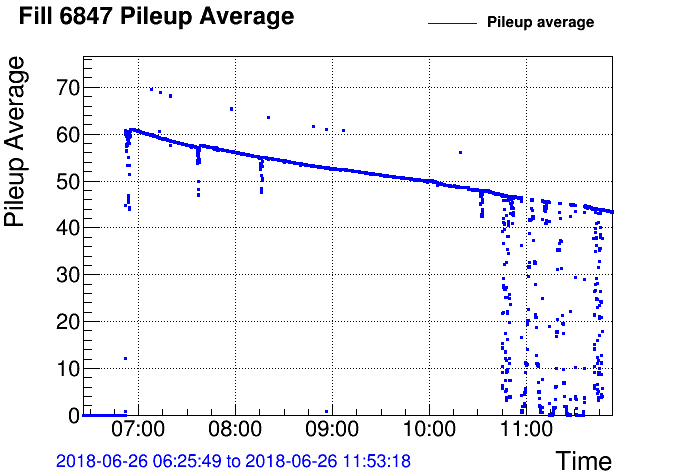
\includegraphics[width=0.55\linewidth]{plots/fill_6847_pileup_avg.png}
    \caption{
      Pile-up profile for LHC fill 6847. Two pile-up scans were performed between 11:00-11:30.
      \label{fig:fillpu6847}
    }
  \end{center}
\end{figure}

\begin{figure}[hbt]
  \begin{center}
    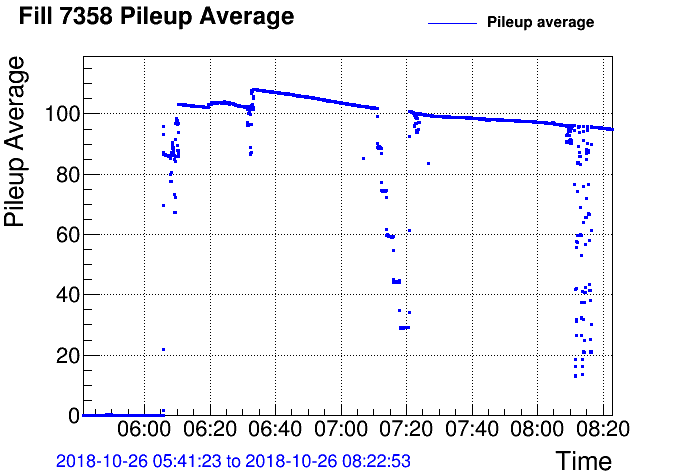
\includegraphics[width=0.55\linewidth]{plots/fill_7358_pileup_avg.png}
    \caption{
      Pile-up profile for LHC fill 7358. A pile-up scan was performed between  07:10-07:20.
      \label{fig:fillpu7358}
    }
  \end{center}
\end{figure}

\clearpage
\begin{figure}[hbt]
  \begin{center}

    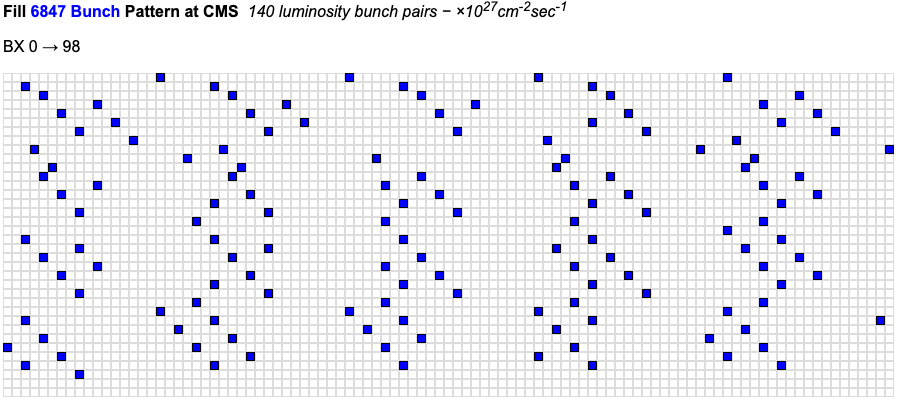
\includegraphics[width=0.99\linewidth]{plots/fillpattern_6847.png}
    \caption{
      Colliding bunch pattern for LHC fill 6847. 
    \label{fig:fill6847pattern}
    }

    \vspace{12pt}
    
    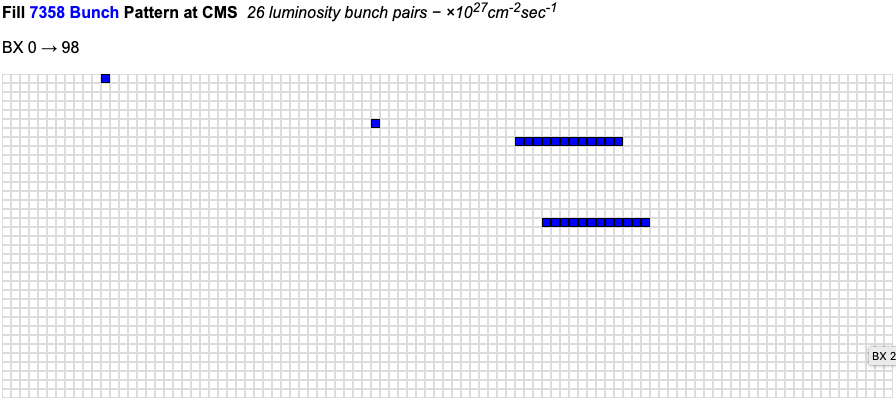
\includegraphics[width=0.99\linewidth]{plots/fillpattern_7358.png}
    \caption{
      Colliding bunch pattern for LHC fill 7358. 
    \label{fig:fill7358pattern}
    }

  \end{center}
\end{figure}

